
%(BEGIN_QUESTION)
% Copyright 2006, Tony R. Kuphaldt, released under the Creative Commons Attribution License (v 1.0)
% This means you may do almost anything with this work of mine, so long as you give me proper credit

Beskriv \textit{Coriolis-effekten}, og hvordan den brukes til å måle fluidstrøm.

\underbar{file i00535}
%(END_QUESTION)





%(BEGIN_ANSWER)

Strømningsinstrumenter basert på Coriolis-effekten bruker et oscillerende rør for å måle massestrøm. Røret drives vanligvis i svingning av en elektromagnetisk ``driver''-spole som får AC-spenning:

$$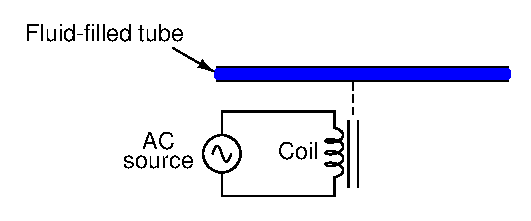
\includegraphics[width=15.5cm]{i00535x01.eps}$$

Når det ikke strømmer væske gjennom røret, oscillerer røret bare fram og tilbake som en anslått gitarstreng:

$$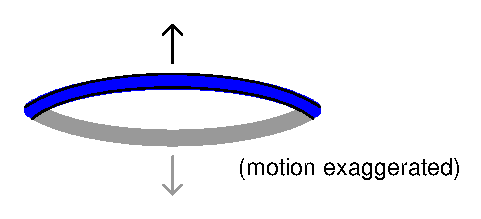
\includegraphics[width=15.5cm]{i00535x02.eps}$$

Når det derimot er strømning fra venstre mot høyre, vil røret vris under oscillasjonen som følge av treghetskrefter. Jo høyere strømning, desto større vridning:

$$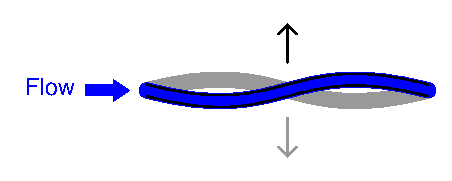
\includegraphics[width=15.5cm]{i00535x03.eps}$$

Ved å måle graden av vridning kan massestrømmen bestemmes. Det er viktig å forstå at det er \textit{massestrøm} som bestemmer styrken på Coriolis-effekten. Hvis fluidets tetthet øker, slik at samme \textit{volumstrøm} tilsvarer høyere massestrøm, vil et ekte massestrømningsinstrument som dette indikere økningen i massestrøm og ikke bli ``lurt'' av at samme antall gallon per minutt (eller annen volum/tid-enhet) passerer.

Nokså interessant har jeg sett applikasjoner der Coriolis-målere ble brukt for å måle \textit{volumstrøm}, ikke massestrøm. Coriolis-måleren ble valgt på grunn av høy nøyaktighet, men råsignalet måtte ``kompenseres'' for å indikere volum i stedet for masse. Denne kompensasjonen ble gjort ved frekvensmåling av det oscillerende røret, der rørets resonansfrekvens er en funksjon av massen innenfor rørets faste volum (altså massetetthet, $\rho$) og rørets fjærkonstant, utledet fra temperaturmåling av rørveggen. Med kjent tetthet gir divisjon av massestrøm (lbm/s) på massetetthet (lbm/ft$^{3}$) volumstrøm (kubikkfot/sekund).

Coriolis-instrumenter er vanligvis svært nøyaktige, og er (teoretisk) upåvirket av temperatur, tetthet, trykk, Reynolds-tall eller andre faktorer som ofte påvirker andre strømningsmåleteknologier. Disse faktorene har målbar effekt på Coriolis-kalibrering (på grunn av strukturelle endringer i måleren), men effektene er i stor grad neglisjerbare.

%(END_ANSWER)





%(BEGIN_NOTES)


%INDEX% Måling, strømning: Coriolis (masse)

%(END_NOTES)

